%\doublespace
\ChNumVar{\fontsize{76}{80}\usefont{OT1}{pzc}{m}{n}\selectfont}

\ChTitleVar{\scshape \raggedleft \LARGE  \bfseries}


\chapter{Consommations d'énergie des data centers} % Main chapter title %
\vspace{3cm}
\minitoc
%\vspace{3cm}
% \begin{center}
%\resizebox{!}{6mm}{\bf \fontfamily{lmss}\selectfont Consommations d'énergie au niveau des data centers}\\
%\end{center}
%\lhead{\normalsize \bf \fontfamily{lmss}\selectfont \@nomChap}

\clearpage



\label{Chapitre1} % For referencing the chapter elsewhere, use \ref{Chapter1} 

%\lhead{Chapitre 1. \emph{Consommations d’énergie}} % This is for the header on each page - perhaps a shortened title




\section{Introduction}
\begin{onehalfspace}
\paragraph{}\lettrine[nindent=1em,lines=3]{L}es énergies fossiles (pétrole, gaz, charbon) ont façonné le monde d’aujourd’hui. Elles sont à l’origine de la révolution industrielle et du développement des transports et ont modelé l’organisation sociale et économique actuelle de l’humanité. Les stocks de pétrole, de gaz et de charbon seront vides d’ici quelques décennies et ne se reconstitueront pas avant plusieurs centaines de millions d’années \cite{WEB46}. Bon gré ou malgré, nous n’avons donc pas d'autres choix que de tendre vers plus de sobriété énergétique, le temps de trouver des alternatives viables aux énergies fossiles. D’autant que l’exploitation intensive de ces ressources carbonées a considérablement augmenté l’effet de serre ces 50 dernières années entraînant un dérèglement climatique global. Ce dérèglement met en danger la survie de l’humanité, notamment en accélérant l’écroulement de la biodiversité.
\paragraph{}Les problèmes liés aux émissions de dioxyde de carbone et à l’énergie font de plus en plus souvent la une des journaux internationaux. Les gouvernements, les associations à but non lucratif et les entreprises réalisent désormais des enquêtes régulières afin d’analyser leur émissions du gaz CO2. Leur objectif est de mesurer l’incidence de leurs activités sur le réchauffement climatique et d’élaborer des plans d’action visant à réduire leurs émissions de dioxyde de carbone.

\end{onehalfspace}
\section{Définition des data centers}
\begin{onehalfspace}
Le data center est un terme anglais qui est employé par les professionnels de l’informatique. Un data center est un bâtiment spécialement conçu pour héberger des équipements informatiques. Ces bâtiments sont découpés en plusieurs salles qu’on appelle des salles blanches. Les grandes entreprises disposent souvent de plusieurs data center pour héberger leurs serveurs. Cependant, de nombreux centre de données sont mutualisés et ils hébergent des serveurs de différents clients.

\end{onehalfspace}
\section{L'impact énergétique des data centers}
\begin{onehalfspace}
L'alimentation électrique est un aspect stratégique pour un cloud data center : sans électricité en quantité suffisante, un data center ne peut pas fonctionner. C'est pour cette raison que les data centers sont construits dans des zones où les infrastructures électriques sont importantes.\medskip 

La consommation d'énergie des salles serveurs ne cesse d'augmenter pour répondre aux besoins notamment des services web. La consommation électrique des data centers a doublé en 5 ans et les études montrent que la tendance s'accélère.\medskip 

La direction informatique se retrouve ainsi au centre de nouveaux enjeux: enjeux financiers comme source de réduction des coûts, enjeux environnementaux en participant à la réduction des émissions de CO$_{2}$. \medskip 

La part de la facture électrique représente 10\% du coût de fonctionnement d'un centre de données. Elle pourrait s'élever très rapidement à 50\% en absence des changements \cite{WEB1}.\medskip \\
Selon une étude IDC, pour 1\$ investit dans le hardware, 1\$ d'énergie sera dépensé \cite{WEB1}.\medskip 

Ces centres qui regroupent les serveurs où sont stockées les données informatiques, sont de véritables gouffres énergétiques. Selon Dalkia\footnote{Dalkia est une entreprise spécialisée dans les services énergétiques, filiale de Veolia Environnement à 66\% et d'Électricité de France à 34\%. Son siège social est situé à Saint-André-lez-Lille, en France.}, un data center de 10.000 $m^{2}$ consomme autant d'énergie qu'une ville de 50.000 habitants.\medskip 

D'après une étude de l'Université de Standford, les quelques 500.000 data centers  existants dans le monde consomment environ 30 milliards de watts d'électricité par an, soit l'équivalent de la production de 30 centrales nucléaires \cite{ref6}.\medskip 

L'énergie dépensée par les centres de stockage des données informatiques est equivalente à 1,5\% de la consommation électrique mondiale. Les data centers seraient également responsables de 2\% des émissions mondiales de CO$_{2}$, soit autant que le trafic aérien mondial.\medskip 

Le poids de la consommation d'énergie des data centers est encore plus important dans les pays développés. selon France Culture\footnote{France Culture est la chaîne de radio culturelle nationale publique française du groupe Radio France.}, en France les data centers consomment 9\% de l’électricité du pays. Les statistiques montrent que le  premier data center construit par Facebook en Europe consomme à lui seul 1\% de l’énergie suédoise.\medskip 

Selon un rapport de l'EPA\footnote{Environmental Protection Agency, Agence américaine de protection de l'environnement \cite{ref3}}, les data centers implantés aux Etats-Unis ont consommé 61 milliards de kilowatt/heures d'électricité en 2006. Ce chiffre représente 1,5 \% de toute l'électricité consommée aux Etats-Unis et un coût de 4,5 milliards de dollars. Les data centers ont été identifiés comme l'un des consommateurs d'énergie qui connaît la croissance la plus rapide. L'EPA exige que le secteur public développe des stratégies pour améliorer l'efficacité énergétique de ses data centers et a fixé un objectif d'amélioration de 20 \% \cite{ref3}. Les data centers du secteur privé, quant à eux, pourraient bien être contraints de respecter sous peu des limites d'émissions de CO$_{2}$.\medskip 
%Les 15 pays qui étaient membres de l’UE avant 2004 se sont engagés à respecter les principes du Protocole de Kyoto. Ils ont convenu de réduire leurs émissions combinées de gaz à effet de serre de 8 \% par rapport à leur niveau de 1990 d’ici 2012(\textit{European Environment Agency, Greenhouse Gas Emission Trends and Projections in Europe 2008, EEA Report No. 5, 2008}). En outre, la Commission Européenne a rédigé un Code de conduite pour les datacenters européens, qui se présente sous la forme d’un ensemble de mesures volontaires d’amélioration de l’efficacité conçu pour définir des normes minimales qui serviront de base à l’établissement d’une réglementation plus contraignante à l’avenir. Son objectif ultime est d’améliorer de 30 \% l’efficacité énergétique moyenne des datacenters.\\

La croissance du secteur étant très importante en raison du développement d'Internet sur appareils mobiles et de l'augmentation des besoins de stockage des entreprises. La demande énergétique liée au data centers va continuer à augmenter fortement.
\end{onehalfspace}
\section{Pourquoi les data centers consomment autant d'énergie ?}
\begin{onehalfspace}
La consommation d’énergie conséquente des data centers s’explique par plusieurs raisons. D'une par, les serveurs de stockage ne peuvent pratiquement jamais être arrêtés pour ne pas perdre les données confiées par les clients des data centers. Ils fonctionnent donc 24 heures sur 24, tous les jours de l'année.
\medskip 

De plus, ces serveurs sont des appareils électroniques de grande taille qui produisent énormément de chaleur. Leur bon fonctionnement est assuré par des systèmes de climatisation très énergivores.\medskip 

Enfin, pour ne pas perdre de données lors d'éventuelles coupures d'électricité, les data centers sont équipés de générateurs de secours fonctionnant au fioul (émetteurs de CO$_{2}$), voire de batteries, qui contribuent à accentuer leur dépense énergétique.
\end{onehalfspace}
\section{Pourquoi réduire la consommation ?}
\begin{onehalfspace}
Suivant la courbe de progression de la performance de calcul \cite{ref2}, la consommation d’énergie des data centers n’a cessé de croître ces dernières années. %\textbf{Cependant, de la même manière que pour les processeurs, nous allons heurter le mur de la consommation. Lorsque le temps était à la course à la miniaturisation il est apparu que la densité de chaleur générée par le composant imposait une contrainte forte sur la densité des transistors. Un parallèle peut être fait avec les clusters et la consommation d'électricité qu'ils génèrent.}\medskip 

Ainsi, les clusters ont augmenté leur nombre de serveurs en même temps que leur puissance. Ce qui nous amène à faire des prédictions pour le futur de la consommation des data centers, qui sont du même ordre que le mur de la miniaturisation des composants. En effet, la miniaturisation croissante des processeurs a dû ralentir le fait de la dissipation de la chaleur insuffisante, et a amené les constructeurs à changer leurs architectures en augmentant le nombre de processeurs ou de cœurs. Si on prévoit la consommation électrique des superordinateurs du top500 \cite{WEB5} en supposant qu'elle croît de façon constante, on arrivera à des clusters d'une consommation de plusieurs centaines de mégawatts ! ce qui nécessite d'avoir un réacteur nucléaire pour alimenter ces supercalculateurs.\medskip 

Il est donc nécessaire de réduire cette consommation par des moyens permettant à la fois de réduire l’énergie demandée et de garder un niveau acceptable de performance. Eteindre systématiquement la moitié des serveurs entrainant  la  réduction de la consommation d’énergie, ça n’est évidemment pas une solution fiable. Ajoutons à cela l’impact environnemental des data center. Décentraliser les opérations locales réduit la consommation d’énergie et l’émission du gaz CO$_{2}$, cela en délocalisant les applications vers des serveurs plus efficaces énergétiquement. Selon un rapport de Greenpeace \cite{WEB4}, la  consommation d’énergie globale des data centers était responsable en 2007 de 116 tonnes de dioxyde de carbone (MtCO2). Ce même rapport estime que ces mêmes émissions pourraient doubler d’ici  2020 pour atteindre 257 MtCO$_{2}$.\medskip

La consommation d’énergie des serveurs n’est pas en effet la seule source d’émission du gaz CO$_{2}$. Il faut aussi prendre en compte le cycle de vie complet d’un serveur, depuis le moment où le serveur est construit jusqu’à son démantèlement. Un serveur sera responsable de plus d’émission du gaz CO2  que sa consommation d’électricité \cite{WEB46}.\medskip 

Enfin, le coût d'électricité de l'exploitation d'un data center peut rapidement devenir important, jusqu’à ce que la consommation d'électricité sur plusieurs années revienne au même prix qu'acheter ce même data center.\medskip 

Que ce soit donc pour des raisons économiques, environnementales ou tout simplement pratiques,
il est intéressant, voire dans certains cas nécessaire, de réduire la consommation énergétique des clouds. Cependant, comme nous allons le voir par la suite, cela ne peut pas se faire de
n'importe quelle façon.
\end{onehalfspace}
\section{Le Power Usage Effectiveness (PUE)}
\subsection{Le PUE : c'est quoi ?}
\begin{onehalfspace}
Le PUE est un indicateur mis au point par le Green Grid pour mesurer l'efficacité énergétique d'un data center. Il est calculé en divisant le total de l'énergie consommée par le data center par le total de l'énergie utilisée par les équipements informatiques (serveur, stockage, réseau). En moyenne les data center français ont un PUE de 2,5 ce qui signifie que pour 1 Watt consommé par l'équipement informatique, il en faut 2,5 Watt à l'entrée du data center. \\
Sans être un indicateur suffisant pour déterminer l'efficience d'un data center, il n'en demeure pas moins qu'un indicateur universellement reconnu \cite{WEB7}.
\end{onehalfspace}
\subsection{Faut-il choisir entre disponibilité du data center et PUE ?}
\begin{onehalfspace}
Les équipements informatiques sont hébergés dans un data center disposant d’une infrastructure complexe (onduleurs, batteries, groupes électrogènes , climatisations, …) destinée à maximiser le taux de disponibilité des équipements qu’il héberge. La norme TIER définie par l’UPTIME Institute \footnote{The Uptime Institute, association américaine, a défini en 1995 une norme permettant d’analyser les topologies mises en œuvre et de délivrer une certification. Cette norme décrit quatre topologies d’infrastructure de sites dont les niveaux croissants d’éléments et de chemins de distribution redondants servent de base de comparaison.} classifie les data centers de 1 à 4. Les data centers de type TIER 1 disposent d’une seule chaîne électrique alors que les data centers de type TIER 4 disposent de 2 chaînes électriques en redondance totale. Par conséquent,  ces derniers assurent une disponibilité statistique de 99,995\%, soit une indisponibilité de 0,5 heure par an contre 99,671\% et 28,8 heures d’indisponibilité statistique annuelle pour ceux de type TIER 1 \cite{WEB7}.\medskip

A l'heure ou le fonctionnement de chaque entreprise est de plus en plus dépendant de l'informatique, la tendance actuelle est de privilégier des data centers avec le niveau de TIER le plus élevé. Sans rentrer dans le débat de la légitimité de cet indice, on constatera tout au moins que l'on attend un taux de disponibilité de plus en plus important \cite{WEB7}.\medskip 

Par voie de conséquence, ce type de data center suppose une infrastructure plus importante qui augmente logiquement le PUE. Ceci est d'autant plus vrai qu'une architecture classique de type TIER 4 impliquant de répartir la charge entre les sources de production électrique. Ceci conduit les onduleurs à être chargés autour de 40\% et donc moins efficients que dans leur plage de fonctionnement de prédilection située autour de 80\%. Ces derniers ayant un moins bon rendement, ils contribuent à dégrader encore le PUE.\medskip 

Il est donc plus facile d’avoir un bon PUE avec un faible niveau de TIER. On voit  bien que cet indicateur n’est pas moins insuffisant  malgré sa pertinence d'un point de vue écologique \cite{WEB7}.
\end{onehalfspace}
La Figure \ref{Cdatacenters}, illustre La consommation électrique dans les data centers.
\begin{figure}[!h]
\begin{center}
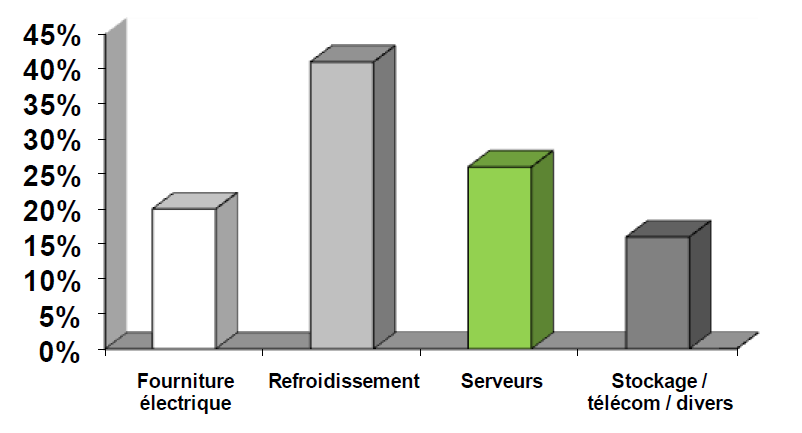
\includegraphics[scale=0.5]{figures/1.png} 
\end{center}
\caption{La consommation électrique dans les data centers}
\label{Cdatacenters}
\end{figure}

\section{Consommations d'énergie au niveau du systèmes de refroidissement}
\begin{onehalfspace}
Comme c'est illustrée dans la Figure 1.1, le refroidissement représente jusqu'à 50\% de la consommation d'énergie totale des data centers et des salles serveurs. Il est donc essentiel de concevoir un refroidissement efficace pour les sites informatiques quelle que soit leur taille.\medskip 

L'électricité consommée par les équipements informatiques est presque entièrement transformée en chaleur
par effet \textit{Joule}. Pour tenir à température constante le matériel, un système de refroidissement est nécessaire.
Sur un ordinateur personnel, ce rôle est tenu par un ou deux ventilateurs. Dans une salle contenant plusieurs
centaines d'équipements informatiques, l'installation d'une climatisation est nécessaire. Les nouveaux data centers déclarent souvent qu'ils utilisent des
sources froides naturelles, généralement de l'air, en complément de la climatisation.\medskip 

Il est possible de récupérer et de valoriser la chaleur produite par les climatisations. Cette chaleur pourrait
être valorisée dans des réseaux de chaleurs locaux dans une logique de filière énergétique locale. Pourtant,
la valorisation de la chaleur dans un réseau de chauffage urbain est rarement mise en œuvre lors de la
construction des data centers
\end{onehalfspace}

\section{Consommations d'énergie au niveau des serveur}
\begin{onehalfspace}
Les serveurs sont les équipements les plus énergétiques dans les data centers, ils consomment environ 40\% d’énergie totale des Data Centers. Ils constituent donc l’une des cibles prioritaires pour la mise en oeuvre des mesures d’économie d’énergie \cite{WEB47}.\medskip 

Pour traiter les données au sein de certains Data Centres, les serveurs n’utilisent que 6\% à 12\% d’énergie qu’ils consomment \cite{ref6}. Un serveur qui n’utilise que 20\% de sa capacité de calcul utilise déjà 70\% de sa puissance électrique maximale. Par ailleurs, une pièce jointe liée à un ancien mail de trois ans doit être stockée sur un serveur qui consomme de l’énergie pour fonctionner même si on  n’utilise plus la pièce jointe.\medskip 

24,7 milliards de dollars sont dépensés chaque année pour le matériel, la maintenance, la gestion, l’alimentation énergétique et le refroidissement des serveurs non utilisés. Cela représente environ le coût des 13 années du programme Apollo\footnote{Coûts du programme Apollo : 25,4 milliards de dollars.}\cite{ref8}.\medskip 

L’énergie consommée pour faire fonctionner ces serveurs non utilisés  compense les émissions du gaz CO$_{2}$ de 6,5 millions de véhicules.\medskip 

Un serveur à haute efficacité énergétique comporte des composants performants d’un point de vue énergétique, tels que les blocs d’alimentation, les processeurs, les disques durs, la mémoire et les connecteurs d’extension. À cette fin, des cartes mères pour serveur, plus efficaces que celles des générations précédentes sont également en cours de développement. L’idée générale est de minimiser les pertes liées à la transformation de courant sur la carte mère. Ces pertes sont  induites par l’écart entre la puissance d’entrée (sortie du bloc d’alimentation) et la puissance au niveau de chacun des composants \cite{WEB47}.


\begin{center}
\begin{tabular}{|c||c|}
\hline
\textbf{Composant} & \textbf{Puissance max (W)} \\
\hline
Processeur & 80 \\
\hline
Mémoire vive & 36 \\
\hline
Disques & 12 \\
\hline
Connecteurs d'extension & 50 \\
\hline
Carte mère & 25 \\
\hline
Ventilateurs & 10 \\
\hline
Alimentation & 38 \\
\hline
\end{tabular}
\captionof{table}{Exemples de puissance absorbée par différents composants}
\label{tab1}
\end{center}


Le tableau \ref{tab1} indique la consommation énergétique approximative de différents composants matériels et montre que les processeurs, les blocs d’alimentation, la mémoire vive et les bus de connecteurs d’extension sont ceux qui absorbent le plus de puissance.
\end{onehalfspace}

%\subsection{Efficacité du processeur}
%\begin{onehalfspace}

%\end{onehalfspace}

\section{Conclusion}
\begin{onehalfspace}
La problématique est donc la suivante : comment réduire la consommation d'énergie des serveurs sans pour autant trop impacter la qualité de service et les performances des applications qui s'exécutent sur le cloud ? Il existe de nombreux moyens pour réduire la facture d'électricité, et un bon nombre de techniques peuvent se faire sans impacter la qualité de service. Cependant, en acceptant une dégradation faible de performance, il est possible de réduire encore plus la puissance consommée par l'infrastructure.\medskip

Dans le prochain chapitre, nous allons présenté quelques techniques nécessaire pour réduire la consommation d'énergie dans les Data centers des Clouds.
\end{onehalfspace}

